OSS possiede una propria base di dati formata da 19 tabelle e 5 viste. Si vogliono mantenere logicamente separati i dati relativi alla PadovaCard.\\

Di seguito venogno riportati lo schema concettuale, lo schema logico e il DDL dell'espansione del database, mentre non viene riportata la struttura del database esistente in quanto non interagirà con le nuove tabelle.\\

Una nota sui nomi delle tabelle è d'obbligo, CackePHP richiede l'utilizzo di una sintassi standard per i nomi delle tabelle, necessaria per effettuare l'accoppiamento model-tabella. Risulta quindi necessario utilizzare nomi inglesi plurali o nomi italiani che terminano per s.
\subsubsection{Modello concettuale}
\begin{figure}[H]
\centering
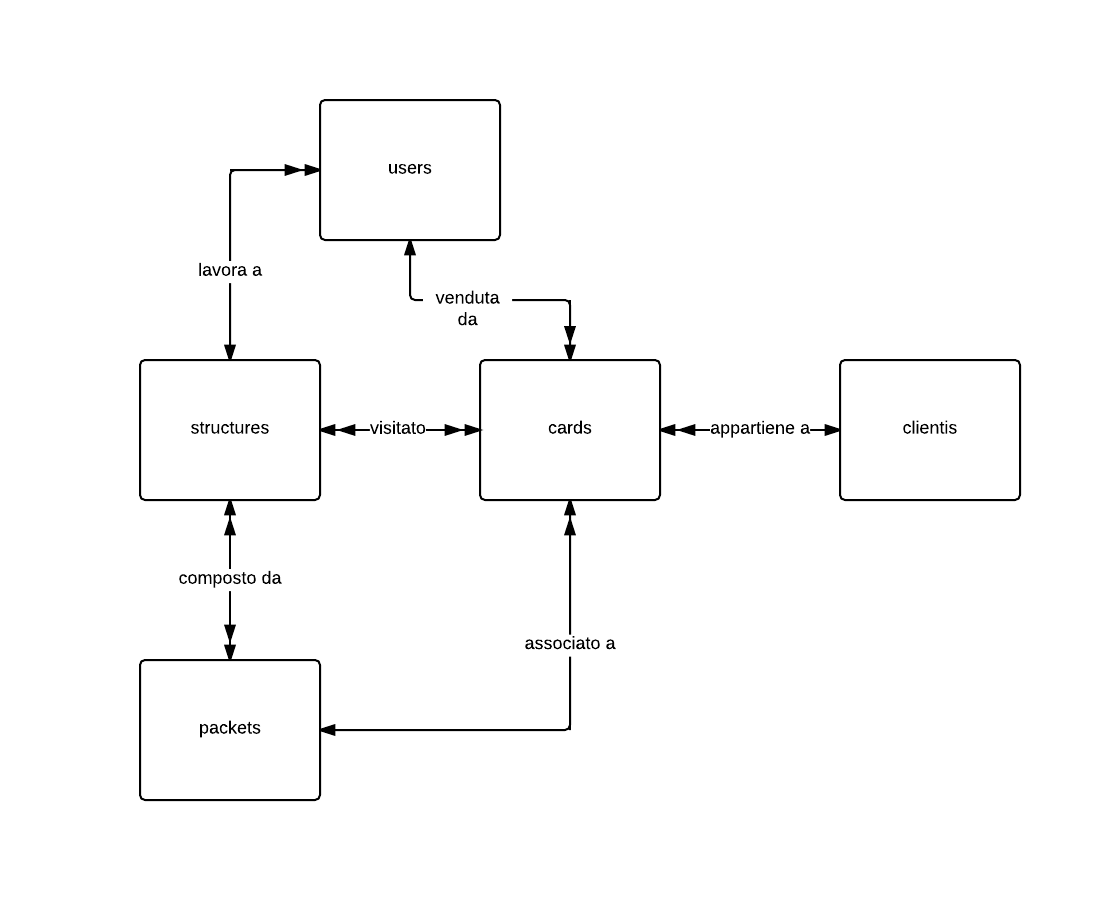
\includegraphics[width=1\textwidth]{images/concettuale.png}
\caption{Modello concettuale della base di dati}
\end{figure}
L'espansione del database già esistente si compone di 3 tabelle, cards, packets e structures mentre tdocumentos e users sono già presenti.
Le nuove tabelle saranno collegate al database esistente tramite tdocumentos e users utilizzando chiavi esterne.\\ \\
\textbf{Tabelle}
\begin{itemize}
\item \textbf{card:} contiene tutte le informazioni sulle PadovaCard;
\item \textbf{packets:} contiene i dati relativi ai pacchetti associabili alla PadovaCard. Ricordiamo che un pacchetto è un insieme di strutture visitabili;
\item \textbf{structures:} contiene i dati su tutte le strutture convenzionate con PadovaCard;
\item \textbf{tdocumentos:} contiene i dati relativi ad un documento di vendita. Un documento corrisponde ad una vendita e può avere al suo interno più articoli, ed essere venduto da un operatore univoco ad un cliente univoco.
\item \textbf{users:} contiene i dati relativi agli operatori e al personale delle strutture. In futuro potrebbe contenere anche quelli relativi agli hotel.
\end{itemize}
\textbf{Relazioni}
\begin{itemize}
\item \textbf{appartiene a:} cards è connessa con una relazione uno a molti a tdocumentos perchè ogni utente può avere una sola PadovaCard attiva, ma più di una non attiva, ogni Padovacard deve essere connessa ad un documento (e quindi ad un cliente);
\item \textbf{associata a:} cards è connessa con una relazione uno a molti a packets perchè ad ogni PadovaCard è associato un solo pacchetto di strutture, mentre un pacchetto può essere associato a più Padovacard;
\item \textbf{composto da:} packets è collegato con una relazione molti a molti a structures in quanto ogni pacchetto è formato da più strutture ed ogni struttura può essere presente su più pacchetti;
\item \textbf{lavora a:} users è collegato con una relazione uno a molti a strcutures per mantenere i dati relativi al personale delle strutture;
\item \textbf{venduta da:} tdocumentos è connesso con una relazione uno a molti ad users in quanto bisogna tener traccia di quale operatore effettua la vendita, un documento e quindi una Padovacard può essere venduta da un solo operatore e un operatore può vendere più PadovaCard;
\item \textbf{visitato:} cards è connesso con una relazione molti a molti a strutture perchè è necessario tener traccia di quali struttre ha visitato l'utente per impedire che con la stessa PadovaCard venga visitata più volte la stessa struttura.


\end{itemize}


\subsubsection{Modello logico-relazionale}
\label{logicorelazionale}

\begin{figure}[H]
\centering
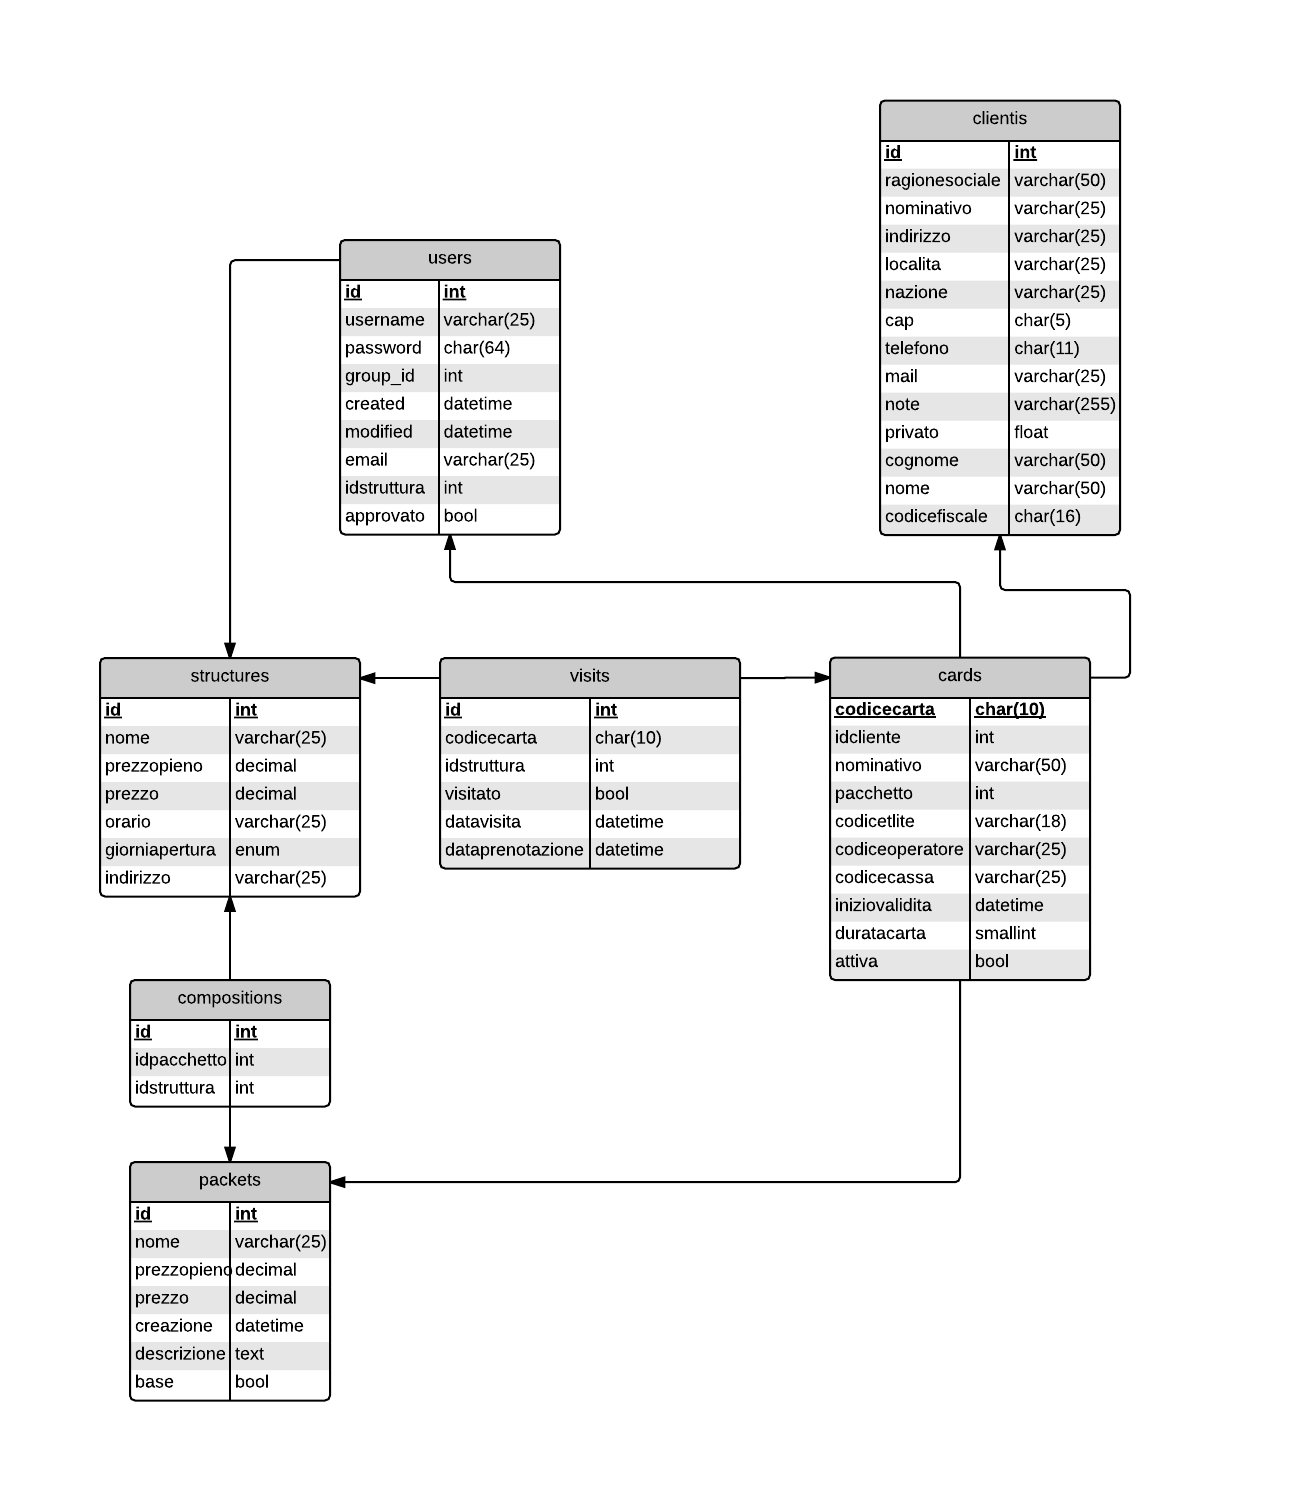
\includegraphics[width=1\textwidth]{images/logico.png}
\caption{Modello logico della base di dati}
\end{figure}
CakePHP prevede che ogni tabella abbia una sola chiave primaria in quanto non supporta chiavi primarie composite, per questo è necessario aggiungere una chiave primaria "di servizio" per CakePHP in tabelle come visite e composizione.\\ \\
\textbf{Note di progettazione}\\ \\
Inizialmente la tabella visits conteneva un campo dataprenotazione che permetteva di gestire la prenotazione a più strutture nel caso in cui in futuro ci fosse tale necessità. \'E altresi vero che la maggior parte dei record avrà Null come valore di dataprenotazione, inoltre in fase di sviluppo si è scoperto che la gestione della data di prenotazione alla \cappella su questa tabella creava notevoli difficoltà. Per questo si è deciso di spostarla sulla tabella cards, limitando la prenotazione alla sola \cappella ma semplificando la logica del software. \\

Attualmente per le password vengono usati campi di tipo char(40) ovvero un campo che può contenere fino ad un massimo di 40 caratteri, sufficienti a contenere l'output della funziona hash \glossario{SHA1} utilizzata di default da CakePHP versione 2.x. Il tirocinante propone di utilizzare un campo char(64) in previsione dell'utilizzo dell'hash \glossario{SHA256}. Tale cambio è motivato nella Sezione \ref{hash}. \\

Nella tabella Users è presente un campo username di tipo varchar(255). Nonostante varchar occupi solamente lo spazio per i caratteri effettivamente scritti, quando vengono create le tabelle temporanee durante le query viene allocata la lunghezza massima. Per questo il tirocinante propone di modificare varchar(255) in varchar(25), più che sufficiente per i valori di tale campo. \\

Nella tabella Users c'è il campo approvato che indica se un iscritto è stato approvato dall'amministratore. Si tratta di un flag 0-1, ma non può essere di tipo bool a causa della funzione Paginate di CakePHP, che non supporta tale tipo. \'E necessario quindi usare un tipo char(1). \\

Clientis contiene i campi cap, telefono e note di tipo varchar(25). Il tirocinante propone di modificare il tipo di cap in char(5), telefono in char(11) e note in varchar(255) in quanto tale valore per varchar è il massimo ottenibile con un solo byte di overhead. Codicefiscale che ora ha tipo varchar(16) viene modificato in tipo char(16). \\

La chiave primaria di Cards è codicecarta, con tipo char(10). Si è scelto di utilizzare codicecarta e non un id auto increment in quanto è univoca e permette di evitare una join durante la lettura di visits. Questo è ottimale in quanto visits sarà la tabella con più query in lettura, mentre si stima la perdita di efficienza nell'uso di char invece di int inferiore al 20\% nel caso peggiore, considerando la lunghezza del char, il fatto che è indicizzato e che il motore usato è \glossario{INNODB}. \\

Sempre in Cards duratacarta è uno smallint. Ad oggi sono previste solo due durate, 48 e 72 ore, per cui un tipo bool sarebbe stato sufficiente ma uno smallint permette di creare più di due tipologie di durata, e di salvare direttamente il numero di ore. \\

La tabella Packets contiene il campo descrizione di tipo text, ritenuto necessario se si vuole salvare qui la descrizione completa della struttura che apparirà nel sito che l'utente adrà a consultare per ottenere le informazioni sulla PadovaCard. \\

Cards contiene il flag attiva che indica se la carta è stata pagata, e se è quindi valida. Questo flag è settato a 0 quando la carta viene creata, quindi a 1 se il pagamento avviene con contanti o carta di credito, mentre viene lasciato a 0 in attesa del pagamento con bonifico. \\

Cards contiene un campo nominativo e un campo iddocument. Iddocument viene utilizzato per collegare la PadovaCard al documento di vendita e quindi all'anagrafica di chi ha effettuato l'ordine, che può essere una persona sia fisica che giuridica. Nominativo contiene il nome del proprietario della PadovaCard e sarà il nome presente nel voucher. Per questo motivo ci potranno essere più PadovaCard attive con lo stesso iddocument mentre il nominativo sarà unico.\\

Per i campi che rappresentano denaro è stato utilizzato il tipo decimal e si è deciso di continuare ad utilizzarlo in quanto non presenta rischi di approssimazione che invece ha il tipo float. \\ \\
\textbf{Tabelle}\\ \\
Nella seguente Sezione verranno descritte nel dettaglio le tabelle che saranno create. Per ogni tabella è fornita una descrizione sul contenuto e un elenco dei suoi campi, comprensivo di tipo e altre note. \\ \\
PK indica che tale campo è \glossario{chiave primaria} della tabella. \\
FK indica che tale campo  è \glossario{chiave esterna} della tabella.\\
\\ \\
CARDS: Contiene tutti i dati relativi alla PadovaCard.
\begin{itemize}
\item codicecarta: char(10) \textit{\textless PK\textgreater}
\item iddocument: int \textit{\textless FK\textgreater}
\item pacchetto: int \textit{\textless FK\textgreater}
\item nominativo: varchar(50)
\item codicetlite: varchar(18)
\item iniziovalidita: datetime
\item duratacarta: smallint
\item attiva: bool
\item datacreazione: datetime
\item minore: bool I minori di 14 anni non necessitano di una propria PadovaCard, ma possono essere collegati a quella di un adulto, con il supplemento di un euro.
\item gratuito: bool Un utente che acquista in internet e vuole ritirare la PadovaCard avrà già pagato in internet e quindi la sua PadovaCard sarà gratuita.
\item dataprenotazione: datetime Data della prenotazione alla \cappella.
\item costo: decimal Il costo della PadovaCard, nonostante sia calcolabile si è preferito mantenerlo salvato in un campo.
\item titolo: char(2) Necessario per la retrocompatibilità con OSS.
\end{itemize}
COMPOSITIONS: Tabella creata dalla relazione "composta da", collega le strutture ai pacchetti.
\begin{itemize}
\item id: int \textit{\textless PK\textgreater}
\item idpacchetto: int \textit{\textless FK\textgreater}
\item idstruttura: int \textit{\textless FK\textgreater}
\end{itemize}
PACKETS: Contiene i dati relativi ai pacchetti, composizioni di strutture visitabili.
\begin{itemize}
\item id: int \textit{\textless PK\textgreater}
\item nome: varchar(25)
\item prezzo48: decimal
\item prezzo72: decimal
\item creazione: datetime Data di creazione del pacchetto
\item descrizione: text
\end{itemize}
STRUCTURES: Contiene i dati relativi alle strutture convenzionate con PadovaCard.
\begin{itemize}
\item id: int \textit{\textless PK\textgreater}
\item nome: varchar(50)
\item prezzopieno: decimal Prezzo della struttura se visitata senza PadovaCard
\item prezzo: decimal Prezzo della struttura visitata con PadovaCard
\item orario: varchar(50)
\item giorniapertura: varchar(25)
\item indirizzo: varchar(25)
\item descrizione text
\end{itemize}
TDOCUMENTOS: COntiene i dati relativi ai documenti di vendita.
\begin{itemize}
\item id: int \textit{\textless PK\textgreater}
\item cliente: int \textit{\textless FK\textgreater}
\item pagamento: varchar(25)
\item datadocumento: date
\item oradocumento: time
\item note: varchar(100)
\item inviomailcliente: float
\item invioemailfornitori: float
\item timestamp: timestamp
\item utente: varchar(25) \textit{\textless FK\textgreater}
\item transazione: varchar(25)
\item ip: varchar(25) 
\item ricevutafiscale: varchar(25)
\item htl: varchar(25)
\item annullato: bool
\end{itemize}
USERS: Contiene i dati riguardanti gli operatori e il personale delle strutture.
\begin{itemize}
\item id: int \textit{\textless PK\textgreater}
\item username: varchar(50)
\item password: char(64)
\item group\_id: int 
\item created: datetime
\item modified: datetime
\item tlite: varchar(25) Codice operativo tlite dell'operatore
\item tlitepc: varchar(25) Codice operativo tlite del pc dell'operatore
\item email: varchar(25)
\item idstruttura int \textit{\textless FK\textgreater}
\item approvato: char(1) Indica se l'utente è approvato, e se quindi può accedere o meno a OSS
\end{itemize}
VISITS: Tabella creata dalla relazione "visitato", tiene traccia di quali strutture sono state visitate da una data PadovaCard, e di eventuali prenotazioni.
\begin{itemize}
\item id INT \textit{\textless PK\textgreater}
\item codicecarta: varchar(10) \textit{\textless FK\textgreater}
\item idstruttura: int \textit{\textless FK\textgreater}
\item visitato: bool
\item datavisita: datetime
\end{itemize}
\textbf{Definizione dello schema logico tramite \glossario{DDL} di MySQL} \\ \\
Le tabelle sono scritte in ordine di creazione nel database, questo per rispettare i vincoli dati dalle chiavi esterne.
\lstset{frame=single}
\begin{center}
\begin{lstlisting}
alter table tdocumentos
	add annullato bool not null de,
    add htl varchar(25);
    
alter table users
	modify column password char(64),
    modify column username varchar(25),
    add email varchar(50),
    add approvato char(1),
    add idstruttura int,
    add tlite varchar(25),
	add tlitepc varchar(25),
    add foreign key (idstruttura) references structures (id);

create table packets(
	id int not null auto_increment,
	nome varchar(25) not null,
    prezzo48 decimal default null,
    prezzo72 decimal default null,
    creazione datetime default null,
	descrizione text default null,
	primary key (id)
)ENGINE=InnoDB DEFAULT CHARSET=utf8; 
	
create table structures(
	id int not null auto_increment,
    nome varchar(50) not null,
    prezzopieno decimal default null,
    prezzo decimal not null,
    orario varchar(50) default null,
    giorniapertura varchar(25) default null,
    indirizzo varchar(25) default null,
    desscrizione text,
	primary key (id)18
)ENGINE=InnoDB DEFAULT CHARSET=utf8;

create table compositions(
	id int not null auto_increment,
    idpacchetto int not null,
    idstruttura int not null,
    primary key (id),
    foreign key (idpacchetto) references packets(id),
    foreign key (idstruttura) references structures(id)
)ENGINE=InnoDB DEFAULT CHARSET=utf8;

create table cards(
codicecarta char(10) not null,
iddocument int not null,
pacchetto int not null,
nominativo varchar(50),
codicetlite varchar(18),
iniziovalidita datetime,
duratacarta smallint not null,
attiva bool default 0,
datacreazione datetime,
minore bool default 0,
gratuito bool default 0,
dataprenotazione datetime,
costo decimal not null,
titolo char(2) not null default 'PD',
foreign key (iddocument) references tdocumentos(id),
foreign key (pacchetto) references packets(id),
primary key (codicecarta)
)ENGINE=InnoDB DEFAULT CHARSET=utf8;

create table visits(
id int not null auto_increment,
codicecarta char(10) not null,
idstruttura int not null,
visitato bool,
datavisita datetime,
foreign key (idstruttura) references structures(id),
foreign key (codicecarta) references cards(codicecarta),
primary key (id)
)ENGINE=InnoDB DEFAULT CHARSET=utf8;
\end{lstlisting}
\end{center}